\documentclass[titlepage]{article}
\usepackage[utf8]{inputenc}
\usepackage{amsmath}
\usepackage{tcolorbox}
\usepackage{tcolorbox}
\usepackage{amssymb}
\usepackage{mdframed} % Add easy frames to paragraphs
\usepackage{xparse} % Add support for \NewDocumentEnvironment
\usepackage{amsthm}
\usepackage{physics}
\usepackage{empheq}
\usepackage{xcolor}
\usepackage{float}
\usepackage[
top    = 2.50cm,
bottom = 2.50cm,
left   = 2.75cm,
right  = 2.75cm]{geometry}
\usepackage{fancyhdr}


\newmdenv[ % Define mdframe settings and store as leftrule
  linecolor=graylight,
  topline=false,
  bottomline=false,
  rightline=false,
  skipabove=\topsep,
  skipbelow=\topsep
]{leftrule}

\NewDocumentEnvironment{example}{O{\textbf{Example:}}} % Define example environment
{\begin{leftrule}\noindent\textcolor{red}{#1}\par}
{\end{leftrule}}

\NewDocumentEnvironment{cs}{O{\textbf{Code Snippet:}}} % Define example environment
{\begin{leftrule}\noindent\textcolor{blue}{#1}\par}
{\end{leftrule}}
\pagestyle{fancy}
\lhead{Algorithms}
\rhead{EPFL/Alp Ozen}


\makeatletter
\renewcommand*\env@matrix[1][*\c@MaxMatrixCols c]{%
  \hskip -\arraycolsep
  \let\@ifnextchar\new@ifnextchar
  \array{#1}}
\makeatother

\newcommand{\tens}[1]{%
  \mathbin{\mathop{\otimes}\limits_{#1}}%
}

\newtheorem{thm}{Theorem}[subsection]
\newtheorem{property}{Property}
\newtheorem{cor}{Corollary}[subsection]
\newtheorem{prop}{[Proposition]}
\newtheorem{rem}{Remark}[subsection]
\newtheorem{definition}{Definition}[subsection]
\newtheorem{exm}{Example}[subsection]
\numberwithin{equation}{subsection}

%useful macros
\newcommand{\Rn}{\mathbb{R}^n}
\newcommand{\Rm}{\mathbb{R}^m}
\newcommand{\ld}{linearly dependent}
\newcommand{\li}{linearly independent}


\title{\textbf{Algorithms}}
\author{Alp Ozen}
\date{Fall 2020 - \textcolor{red}{EPFL}}


\begin{document}

\maketitle
\tableofcontents

\clearpage

\section{Week 1: Insertion sort, and simple analysis}

\textbf{Insertion sort}

\begin{tcolorbox}
\begin{itemize}
  \item Start with an empty hand of data
  \item Open data from left to right, each time placing it in the right order
  \item To find correct position, compare the data at hand with all other sorted data in the stack 
\end{itemize}
\end{tcolorbox}

\begin{cs}
\begin{verbatim}
for j = 2 to A.len
    key = A[j];
    i = j - 1; 
    while i > 0 and A[i] > key 
        A[i + 1] = A[i];
        i = i - 1;
    A[i + 1] = key;
\end{verbatim}

\end{cs}

\begin{example}
Suppose we are given the array $8,2,5,10,1,3$
\\

Iteration 1:
\
j=2 \ key = 2 \ i = 1
\\

8,8
\\

2,8
\\

\ \vdots
\end{example}

Now we naturally ask how one may \textit{prove} the correctness of an algorithm? To do this for insertion sort, we must show the \textbf{loop invariance} of our output array $A$. That is, the array $A$ must remain sorted during the initialization, maintenance and termination of the for loop. It is sorted at initialization because it is essentially an array of a single element. It is sorted at maintenance because each new element appended gets inserted into the correct place hence also why it is sorted at termination. 
\\

Another question to ask is the worst and best case running time of insertion sort. This of course depends on the input array. All lines up to the while loop are executed $n$ many times, $n$ being the length of the array. Then the while loop and the inside of it run some indeterminate $t$ many times. Yet this $t$ is simply how many times we have to shift an element to the right. Thus the best case runtime is $O(n)$ when given an already sorted array and the worst case is $O(n^{2})$ when given an array in reverse order since at each step we do $j-1$ shifts resulting in $\sum_{j=2}^{n}(j-1)$.
\\

The key takeaway from this week should be that an algorithm should both be minimal in its \textit{runtime} while taking up minimal \textit{space}. 

\clearpage
\section{Week 2: Divide & Conquer: Merge sort}

\begin{figure}[H]
    \centering
    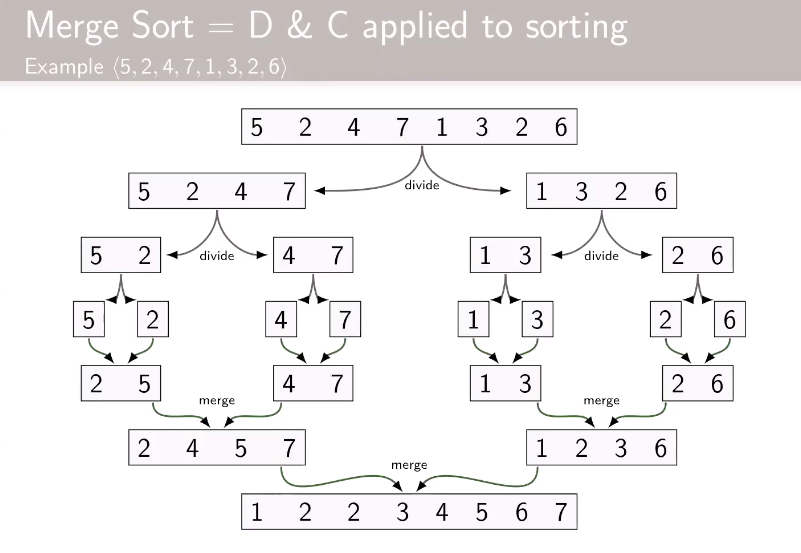
\includegraphics[scale = 0.5]{src/w2.1.png}
    \label{fig:my_label}
\end{figure}

\begin{cs}
\begin{verbatim}
Merge_sort(A,p,r)
if(p<r)
    q = floor((p+r)/2)
    Merge_sort(A,p,q)
    Merge_sort(A,q+1,r)
    Merge(A,q,p,r)
\end{verbatim}

\end{cs}

We now need an algorithm for merging, as it turns out, we can provide a linear time algorithm for this feat. 

\begin{cs}
\begin{verbatim}
Merge(A,p,q,r)
n_1 = q-p+1
n_2 = r-q
for i = 1 to n_1
L[i] = A[p+i-1]
for i = 1 to n_2
R[i] = A[q+i]
L[n_1 + 1] = inf
R[n_2 + 1] = inf
i = 1;
j = 1;
    for k = p to r
        if L[i] =< R[j]
            A[k] = L[i]
            i = i + 1;
        else
            A[k] = R[j]
            j = j + 1 
\end{verbatim}

\end{cs}

\begin{tcolorbox}
\begin{itemize}
  \item Running time of merge is $\Theta(n\log{n})$
\end{itemize}
\end{tcolorbox}

Now let's prove the correctness of the entire algorithm inductively:

\begin{proof}
Let $n = r - p$.
\\

\textbf{Base case:} $n = 0 \implies r = p$ \ hence array is trivially sorted.
\\

\textbf{Inductive step:} Assume true $\forall n \in \{ 0,1, \hdots, k-1\}$ Goal is to show that the procedure works for $n = k$
\\

\textbf{Argument: } Well since we make the recursive calls $Merge-sort(A,p,q)$ and $Merge-sort(A,q+1,r)$ both ranges are in $\{ 0,1, \hdots, k-1\}$ for which we know the procedure works, we are done.
\end{proof}

Let's now derive the runtime of merge-sort but also see a general way to prove the runtime of divide-conquer algorithms. Now let $D(n)$ denote the time to divide the problem, $C(n)$ the time to combine the problem and $T(n)$ the runtime on a problem of size $n$. Then we get the following recurrence: 

$$T(n) = \[ \begin{cases} 
      \Theta(1) & n =1 \\
      aT(\frac{n}{b}) + C(n) + D(n) & \text{otherwise} \\
   \end{cases}
\]$$ 

Now let's simplify. Observe that $D(n) = Theta(1)$ and that $C(n) = \Theta(n)$. Also since we subdivide the problem to size $\frac{n}{2}$ we have $2T(\frac{n}{2}) thus:

$$T(n) = \[ \begin{cases} 
      \Theta(1) & n =1 \\
      2T(\frac{n}{2}) + \Theta(n) & \text{otherwise} \\
   \end{cases}
\]$$ 

Now to solve this recurence there are three possible ways; \textbf{substitution method, recursion tree, master method}. 
\\

We first explore the \textit{substitution method:}
\\

\begin{itemize}
    \item Guess form of solution
    \item Use mathematical induction to find constants and show that solution works 
\end{itemize}

\begin{example}
$$T(n) = 2T(\frac{n}{2}) + cn$$
$$T(n) = 2(2T(\frac{n}{4}) + c\frac{n}{2}) = 4T(\frac{n}{4}) + 2cn$$
$$\vdots$$
This seems a lot like the general form is:
$$2^{k}T(\frac{n}{2^{k}}) + kcn$$
Now since $k = \log_{2}{n}$, a qualified guess for $T(n)$ is that it is $\Theta(n\log{n})$. To prove this supposition, we must show that the expression we obtained is both upper bounded, and lower bounded by $n\log{n}$
\end{example}

\begin{figure}[H]
    \centering
    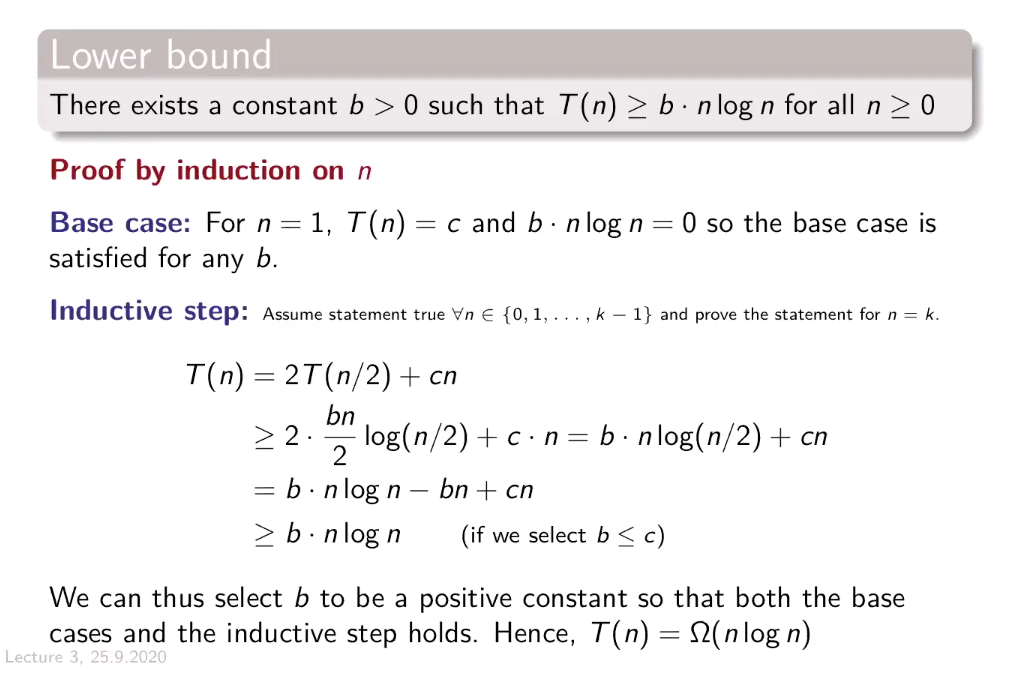
\includegraphics[scale = 0.4]{src/w2.2.png}
    \label{fig:my_label}
\end{figure}

\begin{figure}[H]
    \centering
    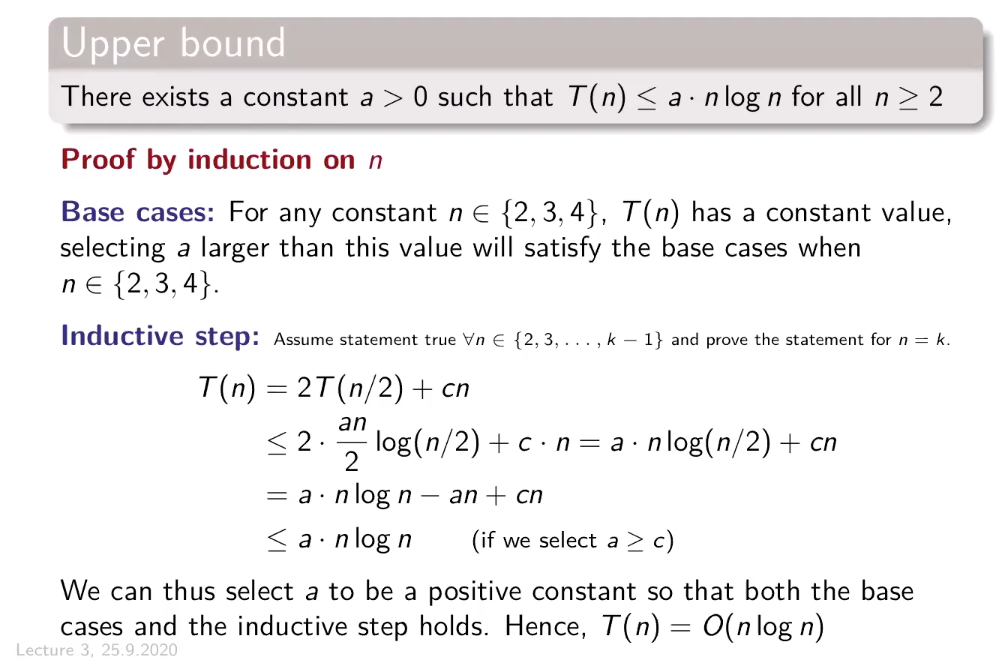
\includegraphics[scale = 0.4]{src/w2.3.png}
    \label{fig:my_label}
\end{figure}



Now to make things more interesting, let's try to arrive at a runtime using a recursion tree approach. 

\begin{figure}[H]
    \centering
    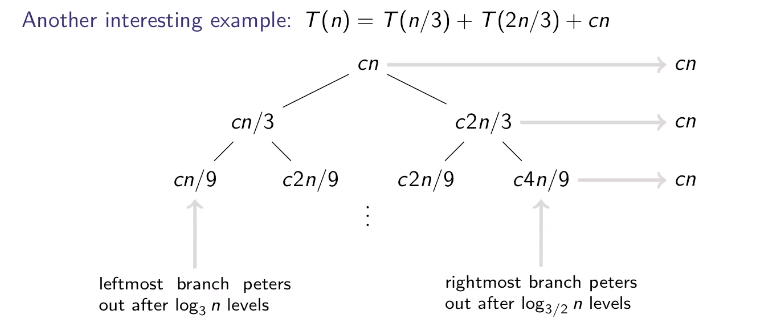
\includegraphics[scale = 0.4]{src/w2.4.png}
    \label{fig:my_label}
\end{figure}

As we can see, each level of the tree contributes some $cn$ steps to the runtime. Now we know that the shortest branch of the tree, the LHS will have $\log_{3}(n)$ branches and the RHS $\log_{\frac{3}{2}}(n)$ branches yielding a cost of $cn\log_{3}(n)$ in the worst case and $cn\log_{\frac{3}{2}}(n)$ in the best case. 
\\

We now present the master theorem without proof:

\begin{theorem}
If we have some recurrence relation of form $$T(n) = aT(\frac{n}{b}) + f(n)$$, then the solution $\Theta(n)$ is either $f(n)$ or $n^{\log_{b}(a)$ depending on which term dominates. 
\end{theorem}




\end{document}